\documentclass[sigconf,nonacm]{acmart}

\usepackage{booktabs}
\usepackage{graphicx}
\usepackage{amsmath}
% acmart already pulls in the AMS symbols through newtxmath, which defines
% \Bbbk; loading amssymb on top of it is a fatal redefinition. Releasing the
% name first is the documented workaround and keeps \checkmark available.
\let\Bbbk\relax
\usepackage{amssymb}
\usepackage{multirow}

% Shrink a table to the column only when it would otherwise overflow. Several
% result tables are generated programmatically and their width depends on the
% data, so hand-tuning \tabcolsep per table would not survive a rerun.
\newcommand{\fitwidth}[1]{%
  \resizebox{\ifdim\width>\columnwidth\columnwidth\else\width\fi}{!}{#1}}

\begin{document}

\title{What Do Hidden Markov Models Learn From Financial Returns?\\
Regime Detection, Redundancy, and Why Conditioning Does Not Help}

\author{Nicholas Reichert}
\affiliation{%
  \institution{Northeastern University}
  \city{Boston}
  \state{Massachusetts}
  \country{USA}}
\email{reichert.n@northeastern.edu}

\begin{abstract}
Applied work reports that conditioning a forecaster on a hidden-Markov-model
regime improves volatility prediction. We tested that claim under strictly
causal filtering, an embargoed train/test boundary, hyperparameters selected
inside the training window, and HAR, GARCH(1,1) and EWMA benchmarks. It fails. A
pooled ridge on identical features wins in 58 of 60 asset-horizon pairs across 20
assets, and no regime variant achieves a significant improvement in 240
Diebold--Mariano tests.

Redundancy explains the failure. Three trailing-volatility features that the
model already reads continuously recover the inferred state with $95.7\%$
accuracy, so gating, shrinkage and feature augmentation each supply estimation
noise and no information.

Running the same pipeline on synthetic data whose generating process we control
locates the failure in the estimator. Two diagnostics that applied work reports
as evidence of regimes fail to identify them. State separation reaches $3.00$ in
a GARCH world containing no discrete states, against $3.15$ under genuine Markov
switching. Reported transition persistence comes mostly from including an
overlapping rolling-volatility emission: fitted to i.i.d.\ noise, the model still
reports substantial persistence, and dropping that one feature removes it.
Because Baum--Welch identifies states by their emission distribution, it recovers
states differing in volatility \emph{level}, which trailing volatility already
reveals, and misses states differing in volatility \emph{dynamics}, which would
carry new information. A de-overlapped diagnostic separates the two worlds and
returns $-0.001$ on SPY, below a GARCH process containing no regimes.

Four ordinary evaluation shortcuts, all four present in our own first
implementation, turn a $-4\%$ result into a significant $+2\%$ one; correcting
the baseline alone flips the sign. We release the pipeline and a checklist.
\end{abstract}

\keywords{volatility forecasting, regime switching, hidden Markov models,
evaluation protocol, data leakage, reproducibility}

\maketitle

%======================================================================
\section{Introduction}
%======================================================================

Financial time series are not stationary. Volatility clusters, correlations
change sign in crises, and the relationship between predictors and returns
appears to shift over time. This motivates \emph{regime-switching} models, in
which a latent discrete state governs the data-generating process
\cite{hamilton1989, ang2012regime}. The natural machine-learning instantiation
is a two-stage pipeline: infer a latent state with a hidden Markov model
\cite{rabiner1989}, then condition a predictor on that state, either by hard
switching between per-regime experts or by soft probability weighting.

The appeal is obvious, the reported results are positive, and the turn toward
machine learning in asset pricing \cite{gu2020empirical} has made such pipelines
easy to assemble. We started in the same place. Our first implementation showed a
clear improvement over a ridge-regression baseline in forecasting SPY volatility.
This paper reports what happened when we tried to make that result robust.

The improvement did not survive. It disappeared once we gave the linear baseline
the same care as the proposed model, and it reversed once we corrected the
target, the train/test boundary and the model-selection step. We are left with a
negative result that decomposes: we can attribute the original effect to
individual methodological shortcuts and say how much each one contributed.

\paragraph{Contributions.}
\begin{enumerate}
  \item \textbf{A causal evaluation, replicated across 20 assets.} We evaluate
    HMM regime-conditioned volatility forecasting under strict online filtering,
    an embargoed walk-forward split, nested hyperparameter selection, and a
    benchmark set that includes HAR \cite{corsi2009}, GARCH(1,1)
    \cite{bollerslev1986}, and EWMA \cite{riskmetrics1996}. Regime conditioning
    provides no significant gain at any horizon, for any asset, under either MSE
    or QLIKE \cite{patton2011}.

  \item \textbf{A decomposition of the null.} We perturb the training partition
    and the prediction-time gate independently, and we test the two ways of using
    the regime signal that avoid gating. The result is an accounting identity: the
    regime signal costs $1.16$ points of RMSE before any gating, gating adds
    $1.59$ more, and correct timing returns $0.69$. Each route loses, and we
    quantify by how much and why.

  \item \textbf{A mechanism.} The three HAR components alone recover the inferred
    state with $95.7\%$ accuracy. The state re-encodes information the model
    already holds, and loses precision doing so, so no method of injecting it
    helps.

  \item \textbf{A simulation study bounding what the estimator can see.} We run
    the same pipeline on data whose generating process we control. The standard
    descriptive diagnostics fail to distinguish a world with regimes from one
    without. Overlapping-window emissions manufacture most of the reported
    transition persistence, which survives even on i.i.d.\ noise. And maximising
    emission likelihood recovers states differing in volatility level while
    missing states differing in volatility dynamics, so the estimator finds the
    regimes least worth conditioning on and misses the ones that would help.

  \item \textbf{Equivalence bounds.} We report what size of improvement the data
    exclude, rather than reporting only a failure to reject. In the median
    asset-horizon pair, no improvement of any size survives at 95\%.

  \item \textbf{Robustness on three further axes.} The null holds under
    gradient-boosted experts, under a Model Confidence Set that weighs all
    competitors at once, and under a decision-relevant loss. That last case is the
    one place where the choice of loss function changes the picture: the regime
    models become indistinguishable from the pooled ridge instead of trailing it,
    while the regime-\emph{free} benchmarks stay significantly ahead of both.

  \item \textbf{A protocol ablation.} Starting from our own first implementation,
    we measure how much apparent improvement each of four evaluation shortcuts
    produces, and show that they compound: together they turn a $-4\%$ result into
    a statistically significant $+2\%$ one.

  \item \textbf{Seed sensitivity.} The spread across HMM random initializations
    alone matches the reported effect size. Applied regime-switching work
    under-appreciates this.

  \item \textbf{A reproducible pipeline and a checklist} for future work in this
    area.
\end{enumerate}

Two things we do \emph{not} claim. Market regimes may well exist, and
regime-switching models have documented value in asset allocation and risk
management \cite{guidolin2007}. Our claim covers this task, this model class and
this benchmark set: the reported forecasting gains come from the evaluation
rather than from the method, and the diagnostics we propose cost little enough to
run as standard.

%======================================================================
\section{Related Work}
%======================================================================

\paragraph{Regime switching.}
Hamilton's Markov-switching autoregression \cite{hamilton1989} established the
econometric template. Subsequent work applies regime switching to asset
allocation \cite{guidolin2007} and documents its role in explaining return
predictability \cite{ang2012regime, timmermann2000}. Most of this literature is
in-sample or uses smoothed (two-sided) state estimates; our concern is the
strictly causal, out-of-sample forecasting case.

\paragraph{Volatility forecasting.}
The benchmark set decides this comparison. GARCH \cite{engle1982,
bollerslev1986} remains hard to beat \cite{hansen2005forecast}, and the HAR
model \cite{corsi2009} is the standard reference for realized volatility, whose
long-memory behavior it captures with three lagged components. Andersen and
Bollerslev \cite{andersen1998} traced the apparent poor performance of volatility
models to the use of squared daily returns as the evaluation proxy; Patton
\cite{patton2011} characterized which loss functions survive such proxy noise,
which is why we report both MSE and QLIKE.

\paragraph{Evaluation and leakage.}
Our methodological concerns are not new. L\'opez de Prado \cite{lopezdeprado2018}
introduced purging and embargoing for financial cross-validation. Bailey et al.
\cite{bailey2014} formalized backtest overfitting, and Harvey et al.
\cite{harvey2016} argued for higher significance thresholds given the volume of
tested strategies. Kaufman et al. \cite{kaufman2012leakage} give the general
taxonomy of leakage into which our embargo and nested-selection corrections fall. Welch and Goyal \cite{welch2008} performed the canonical
re-evaluation of equity-premium predictors and found most did not survive
out-of-sample. Outside finance, Ferrari Dacrema et al. \cite{dacrema2019} showed
that weak baselines account for most reported progress in neural recommendation,
Makridakis et al. \cite{makridakis2018} made the analogous point for ML
forecasting, and Kapoor and Narayanan \cite{kapoor2023leakage} document leakage
as a cross-disciplinary reproducibility problem. Our contribution is to run this
style of audit on the specific, popular case of HMM-based regime-conditioned
forecasting, and to attribute the effect to individual protocol choices rather
than reporting a null alone.

%======================================================================
\section{Problem Setup}
%======================================================================

\subsection{Data}

We use daily SPY (S\&P 500 ETF) OHLCV data from February 2005 to July 2026,
obtained from Yahoo Finance and adjusted for splits and dividends. Let
$p_t$ be the adjusted close and $r_t = \log p_t - \log p_{t-1}$ the daily log
return. After feature construction and the removal of warm-up and trailing rows
the sample contains $5{,}391$ trading days, of which $3{,}771$ (February 2011 to
February 2026) are used for out-of-sample evaluation.

\subsection{Targets}

The forecasting target is realized volatility over the next $h$ days,
\begin{equation}
  y_t^{(h)} \;=\; \mathrm{RV}_{t+1:t+h} \;=\; \sqrt{\frac{1}{h}\sum_{i=1}^{h} r_{t+i}^2},
  \qquad h \in \{1, 5, 20\}.
  \label{eq:target}
\end{equation}
For $h=1$ this reduces to $|r_{t+1}|$, so the family nests the single-day
absolute-return target.

This definition deserves emphasis because the error it guards against is easy to
make and hard to see. A similar-looking definition,
$\tilde{y}_t^{(h)} = |r_{t+h}|$, gives the absolute return of a \emph{single} day
$h$ steps ahead. It aliases: $\tilde{y}^{(1)}$, $\tilde{y}^{(5)}$ and
$\tilde{y}^{(20)}$ are the same series at different lags. One diagnostic exposes
it. Their sample standard deviations are $0.009186$, $0.009185$ and $0.009188$,
identical to four significant figures, whereas the aggregated targets in
Eq.~\eqref{eq:target} give $0.009186$, $0.007508$ and $0.006837$, declining with
$h$ as aggregation requires. Under the aliased definition, varying $h$ varies the
lead time of one unchanged and very noisy prediction problem. We report results
for both. The aliased variant forms the first stage of the protocol ablation in
Section~\ref{sec:protocol}.

\subsection{Features}

All features at time $t$ use information available at $t$: lagged returns
$r_{t-1},\dots,r_{t-20}$; rolling means and standard deviations of returns over
$5$, $10$ and $20$ days; log volume change and rolling volume $z$-scores; and
Wilder's RSI. We additionally include the three HAR components
\begin{equation}
  \mathrm{RV}^{(w)}_t = \sqrt{\tfrac{1}{w}\textstyle\sum_{i=0}^{w-1} r_{t-i}^2},
  \qquad w \in \{1, 5, 22\},
\end{equation}
so that every model in the comparison, including the regime-conditioned one, has
access to the information the HAR benchmark uses. The final feature set has 35
columns.

%======================================================================
\section{Method}
%======================================================================

\subsection{Causal regime inference}

We fit a Gaussian HMM with $K$ states and diagonal covariances on the
three-dimensional emission vector $x_t = (r_t,\, |r_t|,\, \mathrm{RV}^{(20)}_t)$,
standardized using training-window statistics only. Parameters
$(\pi, A, \{\mu_k, \Sigma_k\})$ are estimated by Baum--Welch on the training
window.

The regime probability used at prediction time is the \emph{filtered} posterior
\begin{equation}
  \gamma_t(k) \;=\; \Pr\!\left(z_t = k \mid x_{1:t}\right),
\end{equation}
computed by the forward recursion in log space,
\begin{equation}
  \log\alpha_t(k) \;=\; \log p(x_t \mid z_t{=}k) +
  \log\!\!\sum_{j} \exp\!\big(\log\alpha_{t-1}(j) + \log A_{jk}\big),
\end{equation}
normalized at each step. Regime-switching pipelines leak here more than anywhere
else. The smoothed posterior $\Pr(z_t = k \mid x_{1:T})$ returned by a standard
\texttt{predict\_proba} call, and the Viterbi path returned by \texttt{predict},
both condition on the \emph{entire} sequence including the future, so forming a
forecast at time $t$ from either one uses data the forecaster cannot have. We
implement the forward filter ourselves, and we warm-start the test-window filter
from the final training-window belief $\alpha_{T_{\text{train}}}$ instead of
resetting it to $\pi$, matching what someone running the model in real time
would hold.

\subsection{Label switching across folds}

Baum--Welch state indices are arbitrary: nothing ties ``state 0'' in one fit to
``state 0'' in the next. Since we refit the HMM on every walk-forward window,
concatenating raw state labels across folds interleaves different meanings. The
symptom hides well. Forecasts survive intact, because within a fold we fit and
apply the experts consistently, but every per-regime table and regime-shading
plot then shows apparent regime changes at fold boundaries that are pure
relabelling.

We therefore sort states after each fit by the mean of their volatility emission,
making state $0$ the calmest and state $K-1$ the most volatile. This relabels and
does nothing else: the likelihood, the filtered posteriors and every forecast
stay the same, while regime identities become comparable across folds.

\subsection{Regime-conditioned prediction}

Given filtered probabilities, we fit one ridge expert per regime. Training rows
are assigned to expert $k$ by $\arg\max_k \gamma_t(k)$; regimes with fewer than
$200$ training rows fall back to a globally fitted expert. Predictions combine
the experts either by hard switching,
$\hat{y}_t = f_{\arg\max_k \gamma_t(k)}(x_t)$, or by soft weighting,
$\hat{y}_t = \sum_k \gamma_t(k) f_k(x_t)$.

Each expert is a standardized ridge whose penalty we choose by generalized
cross-validation on its own training subsample. Fairness depends on this.
Feature standard deviations in our set span four orders of magnitude, from
$2.3\times10^{-3}$ for a 20-day mean return to $11.4$ for RSI, so a fixed penalty
on unscaled inputs shrinks some coefficients far harder than others. Handicap a
baseline that way and it stops testing anything.

\subsection{Factorized ablations}
\label{sec:ablations}

A single ``shuffle the regimes'' control answers two questions at once and
separates neither. We therefore perturb the training partition and the
prediction-time gate independently, giving the five arms in
Table~\ref{tab:ablation-design}.

\begin{table}[t]
\caption{Ablation design. ``true'' uses filtered probabilities; ``shuffle''
applies a random time permutation, preserving the marginal distribution of
regime probabilities but destroying their alignment with the market; ``single''
puts all mass on one state.}
\label{tab:ablation-design}
\small
\begin{tabular}{llll}
\toprule
Arm & Train gate & Test gate & Isolates \\
\midrule
\textsc{normal}         & true    & true    & full model \\
\textsc{gate\_shuffle}  & true    & shuffle & value of regime \emph{timing} \\
\textsc{expert\_shuffle}& shuffle & true    & value of regime \emph{experts} \\
\textsc{both\_shuffle}  & shuffle & shuffle & conventional shuffle control \\
\textsc{single}         & single  & single  & pooled ridge (control) \\
\bottomrule
\end{tabular}
\end{table}

\textsc{gate\_shuffle} carries the most weight. We train the experts on genuine
regimes, then hand the model a probability vector drawn from the correct marginal
distribution but attached to the wrong day. If knowing \emph{which regime we are
in today} matters, this arm has to degrade.

We fell into one design trap worth naming. An earlier version of this ablation
suite included a ``uniform gate'' arm meant to remove regime information while
keeping the mixture structure. Since we assign experts by $\arg\max$, a uniform
probability vector selects state $0$ for every row, so that arm collapsed to a
single globally fitted expert and returned numbers identical to the pooled-ridge
control. It looked like an informative ablation and duplicated one we already
had.

%======================================================================
\section{Evaluation Protocol}
\label{sec:protocol-def}
%======================================================================

\paragraph{Walk-forward splits.}
We use a rolling origin: six years of training (about $1{,}500$ observations)
followed by one year of testing, advanced one year at a time, giving $15$ folds
spanning February 2011 to February 2026. The HMM and all model parameters are
refit on each training window.

\paragraph{Embargo.}
Since $y_t^{(h)}$ depends on returns through $t+h$, the final $h$ rows of any
training window carry targets that extend into the test period. We purge them
\cite{lopezdeprado2018}. Skip this step and at $h=20$ the model trains on twenty
observations whose labels come in part from the data about to evaluate it.

\paragraph{Nested selection.}
We select the number of regimes $K \in \{2,3,4\}$ and the gating rule, hard or
soft, \emph{within} each training window, on a trailing 25\% validation block
that we embargo from the inner training portion. We then refit the selected
configuration on the full training window and apply it to the test fold. This
separates what the method achieves from the best of six out-of-sample numbers.

\paragraph{Metrics.}
We pool predictions across folds and report RMSE and QLIKE
\cite{patton2011},
$\mathrm{QLIKE} = \frac{\sigma^2}{\hat\sigma^2} - \log\frac{\sigma^2}{\hat\sigma^2} - 1$,
evaluated on variances. MSE and QLIKE are the two loss families that remain
robust to noise in the volatility proxy, so a ranking that holds under both
cannot be a proxy artifact. QLIKE diverges as $\hat\sigma \to 0$; we floor
forecasts at the 1st percentile of realized values for reporting only.

\paragraph{Significance.}
We use the Diebold--Mariano test \cite{dieboldmariano1995} with a
Newey--West \cite{neweywest1987} long-run variance at lag $h-1$, since
overlapping targets make the loss differential autocorrelated by construction,
and the Harvey--Leybourne--Newbold \cite{harvey1997} small-sample correction.
Because each model is compared against several alternatives we apply a
Holm--Bonferroni correction within each target.

%======================================================================
\section{Results}
\label{sec:results}
%======================================================================

\subsection{Main comparison}

\begin{table}[t]
\caption{Pooled out-of-sample performance on realized-volatility targets, 15 walk-forward folds, Feb 2011--Feb 2026, n=3771. Lower is better. Best per column in \textbf{bold}. Markers report a Holm-corrected Diebold--Mariano test of the regime model against that baseline at the 5\% level: $\ast$ the regime model is significantly better, $\dagger$ significantly worse. The regime model significantly beats only the trivial baselines, and significantly loses to the pooled ridge. QLIKE diverges for near-zero forecasts, which is why the zero and random-walk rows are orders of magnitude above the rest.}
\label{tab:main}
\small
\setlength{\tabcolsep}{4pt}
\fitwidth{%
\begin{tabular}{lrrrrrr}
\toprule
& \multicolumn{2}{c}{$h=1$} & \multicolumn{2}{c}{$h=5$} & \multicolumn{2}{c}{$h=20$} \\
\cmidrule(lr){2-3}\cmidrule(lr){4-5}\cmidrule(lr){6-7}
Model & RMSE & QLIKE & RMSE & QLIKE & RMSE & QLIKE \\
\midrule
Zero & 0.010847$^{\ast}$ & 1.39e+04 & 0.010850$^{\ast}$ & 37.7831 & 0.010852$^{\ast}$ & 8.3736 \\
Train mean & 0.008423$^{\ast}$ & 2.7844 & 0.007042$^{\ast}$ & 1.2120 & 0.006389$^{\ast}$ & 0.8798 \\
Random walk (RV) & 0.009436$^{\ast}$ & 148.9 & 0.005395 & 1.0204 & 0.005706 & 0.6026 \\
EWMA / RiskMetrics & 0.007263 & 1.8569 & 0.005234 & 0.5626 & 0.005061 & 0.5077 \\
HAR & 0.007133 & 1.8414 & 0.004990 & 0.5362 & 0.004967 & 0.4663 \\
GARCH(1,1) & 0.007052 & \textbf{1.7780} & 0.004884 & \textbf{0.5159} & 0.004913 & 0.4725 \\
Ridge (pooled) & \textbf{0.006968}$^{\dagger}$ & 2.1185 & \textbf{0.004719} & 0.5585 & \textbf{0.004867}$^{\dagger}$ & \textbf{0.4642} \\
\midrule
Regime-conditioned (HMM) & 0.007225 & 4.7700 & 0.004925 & 0.5975 & 0.005035 & 0.4963 \\
\bottomrule
\end{tabular}%
}
\end{table}


Table~\ref{tab:main} reports pooled out-of-sample performance.

A pooled ridge on the same features beats the regime-conditioned model at every
horizon, and significantly so at $h=1$ and $h=20$ after we correct for multiple
comparisons. The regime model never beats HAR, GARCH(1,1) or EWMA under either
loss at any conventional level. It beats the zero forecast, the training mean,
and at $h=1$ the random walk in realized volatility. Those are the trivial
benchmarks, and they reproduce the original result in miniature: pick a weak
enough comparison and the method looks convincing.

The two losses disagree about which benchmark ranks first, and the disagreement
helps. GARCH(1,1) wins on QLIKE at $h=1$ and $h=5$, matching
\cite{hansen2005forecast}; the feature-rich ridge wins on RMSE everywhere and on
QLIKE at $h=20$. QLIKE punishes under-prediction hard, favouring the
conditional-variance models that hold forecasts away from zero, while RMSE
rewards the model fitted to minimize squared error. The regime model loses under
\emph{both}, which is what leaves the conclusion independent of the loss we chose.

One implementation check: \textsc{regime\_single}, the ablation arm that
collapses the mixture to one expert, produces predictions bitwise identical to
the pooled ridge at every horizon, confirming that the mixture machinery reduces
correctly. Every other regime arm scores worse.

\subsection{Tracing the regime signal}

\begin{table}[t]
\caption{Ablation of the regime signal (realized-volatility targets). $\Delta$ is RMSE relative to the \textsc{single} pooled-ridge control, in percent; negative would mean the arm beats the control. Shuffling the gate in time does not degrade the model: at $h=1$ and $h=5$ it improves it. If knowing the current regime mattered, the \textsc{gate\_shuffle} row would have to be worse than \textsc{normal}, and it is not.}
\label{tab:ablation}
\small
\setlength{\tabcolsep}{4pt}
\begin{tabular}{lrrrrrr}
\toprule
& \multicolumn{2}{c}{$h=1$} & \multicolumn{2}{c}{$h=5$} & \multicolumn{2}{c}{$h=20$} \\
\cmidrule(lr){2-3}\cmidrule(lr){4-5}\cmidrule(lr){6-7}
Arm & RMSE & $\Delta$\% & RMSE & $\Delta$\% & RMSE & $\Delta$\% \\
\midrule
\textsc{normal} (full model) & 0.007225 & +3.69 & 0.004925 & +4.37 & 0.005035 & +3.45 \\
\textsc{gate\_shuffle} & 0.007106 & +1.98 & 0.004844 & +2.65 & 0.005090 & +4.58 \\
\textsc{expert\_shuffle} & 0.007044 & +1.09 & 0.004785 & +1.39 & 0.004925 & +1.20 \\
\textsc{both\_shuffle} & 0.007144 & +2.53 & 0.004765 & +0.97 & 0.004891 & +0.50 \\
\textsc{single} (pooled ridge) & 0.006968 & +0.00 & 0.004719 & +0.00 & 0.004867 & +0.00 \\
\bottomrule
\end{tabular}
\end{table}


Table~\ref{tab:ablation} applies the design of Section~\ref{sec:ablations} and
carries the central diagnostic. On SPY, \textsc{gate\_shuffle} hands the model
regime probabilities attached to the wrong day and costs nothing in RMSE against
\textsc{normal}. At $h=1$ and $h=5$ it scores \emph{better}.

Read alone, this would make regime timing worthless. The cross-asset evidence in
Section~\ref{sec:multiasset} overturns that reading, and we report it here to
warn against drawing mechanism conclusions from one series: pooled over 60
asset-horizon pairs, correct timing carries a small but detectable benefit. SPY
lands among the cases where it does not.

Both readings agree on the underlying picture. The regime label restates trailing
realized volatility at coarse resolution, and the feature set already carries that
as $\mathrm{RV}^{(1)}$, $\mathrm{RV}^{(5)}$ and $\mathrm{RV}^{(22)}$. A
three-level discretization of a variable the model reads continuously adds
little, and fragmenting the training data across experts to exploit it costs more
than it adds. Section~\ref{sec:multiasset} puts numbers on both sides of that
trade.

\subsection{Protocol ablation}
\label{sec:protocol}

\begin{table}[t]
\caption{Protocol ablation. Improvement of the regime-conditioned model over its \emph{matched} pooled-ridge baseline, as four evaluation shortcuts are removed cumulatively. Positive means the regime model looks better. $p$ is a HAC-corrected Diebold--Mariano test against that baseline. At $h=1$ the aliased and realized-volatility targets coincide by construction, so P3 and P4 are identical.}
\label{tab:protocol}
\small
\setlength{\tabcolsep}{3pt}
\fitwidth{%
\begin{tabular}{llrrrrrr}
\toprule
& & \multicolumn{2}{c}{$h=1$} & \multicolumn{2}{c}{$h=5$} & \multicolumn{2}{c}{$h=20$} \\
\cmidrule(lr){3-4}\cmidrule(lr){5-6}\cmidrule(lr){7-8}
& Correction applied & $\Delta$\% & $p$ & $\Delta$\% & $p$ & $\Delta$\% & $p$ \\
\midrule
P0 & our original implementation & +1.93 & $<$0.001 & +1.25 & 0.001 & +0.63 & 0.183 \\
P1 & + tuned/standardized baseline & -1.03 & 0.041 & -0.37 & 0.123 & -0.23 & 0.368 \\
P2 & + train/test embargo & -1.06 & 0.036 & -0.34 & 0.152 & -0.19 & 0.447 \\
P3 & + nested selection & -3.69 & 0.001 & -1.02 & 0.004 & -0.76 & 0.014 \\
P4 & + realized-vol target & -3.69 & 0.001 & -4.37 & 0.028 & -3.45 & $<$0.001 \\
\bottomrule
\end{tabular}%
}
\end{table}


\begin{figure}[t]
  \centering
  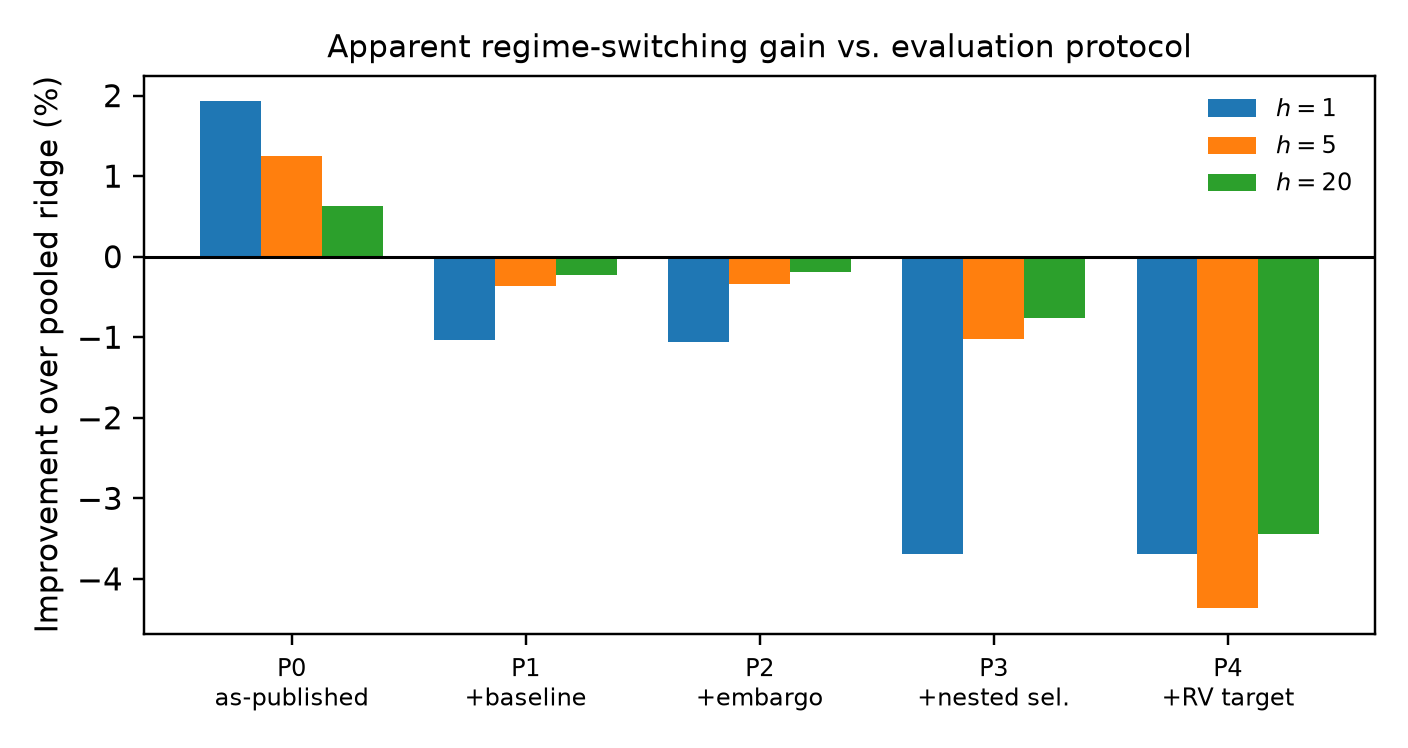
\includegraphics[width=\columnwidth]{figures/protocol_ablation.png}
  \caption{The apparent gain from regime conditioning as a function of the
  evaluation protocol, not of the model. The model is identical in every bar;
  only the protocol changes.}
  \label{fig:protocol}
  \Description{Grouped bar chart of the regime model's improvement over its baseline at five protocol stages, for three horizons. Bars are positive at stage P0 and negative at every later stage.}
\end{figure}

Table~\ref{tab:protocol} and Figure~\ref{fig:protocol} trace the improvement of
the regime model over its matched pooled-ridge baseline as four methodological
choices are corrected in sequence. The model is unchanged throughout; only the
protocol moves.

P0, the starting point, is our own first implementation, written before we
applied any correction in this paper. It reconstructs no published study, and we
make no claim that any particular paper combines all four choices. Our claim is
narrower and more useful: each of the four is easy to make, each survived our own
code review, and together they produce a significant positive result for a method
that does not work.

P0 uses the aliased target, an unstandardized fixed-penalty baseline, no embargo,
and $K$ and the gating rule chosen by out-of-sample score. Under it the regime
model improves on its baseline by $1.9\%$ at $h=1$ and $1.3\%$ at $h=5$, both
significant at the 1\% level. Correcting the baseline alone (P1) flips the sign at
every horizon. Adding the embargo (P2) changes little here. At these horizons the
leak is real but small, and we keep it because nobody can know its size in
advance, not because it dominates. Nested selection (P3) removes a further $0.6$
to $2.6$ percentage points, the largest single correction. The corrected target
(P4) leaves the regime model between $3.4\%$ and $4.4\%$ behind the pooled ridge,
significantly so at every horizon.

They compound for a reason. All four widen the flexibility of the proposed model
relative to its benchmark, so their effects share a sign, which is also why none
of them looks alarming alone. The literature documents each failure mode
separately: leakage across a train/test boundary \cite{lopezdeprado2018,
kapoor2023leakage}, selection reported as evaluation \cite{bailey2014,
harvey2016}, and under-specified baselines \cite{dacrema2019}. The interaction
turns a $-4\%$ result into a significant $+2\%$ one, and a checklist applied one
item at a time will miss interactions.

\subsection{Cross-asset replication}
\label{sec:multiasset}

\begin{table}[t]
\caption{Cross-asset replication. Each cell is the out-of-sample RMSE improvement of the regime-conditioned model over the pooled ridge fitted on identical features, in percent; positive would favour regime conditioning. $^{\dagger}$ marks a Diebold--Mariano rejection at the 5\% level, always in the direction of the pooled ridge. Assets are sorted by mean trailing volatility.}
\label{tab:multiasset}
\small
\setlength{\tabcolsep}{4pt}
\fitwidth{%
\begin{tabular}{llrrrr}
\toprule
Ticker & Class & Vol & $h{=}1$ & $h{=}5$ & $h{=}20$ \\
\midrule
HYG & High yield credit & 0.0048 & -0.69 & -3.87 & -3.38 \\
FXE & EUR/USD & 0.0051 & -0.20 & -2.35$^{\dagger}$ & -2.42 \\
TLT & Long treasuries & 0.0083 & -1.07$^{\dagger}$ & -1.14 & -3.44 \\
SPY & US large cap & 0.0096 & -3.69$^{\dagger}$ & -4.37$^{\dagger}$ & -3.45$^{\dagger}$ \\
KO & Single name (staples) & 0.0098 & -2.48$^{\dagger}$ & -7.53$^{\dagger}$ & -6.15 \\
GLD & Gold & 0.0102 & -0.81$^{\dagger}$ & -2.86$^{\dagger}$ & -3.35$^{\dagger}$ \\
EFA & Developed ex-US & 0.0108 & -1.16 & -2.83$^{\dagger}$ & -6.04$^{\dagger}$ \\
QQQ & US tech-heavy & 0.0117 & -0.66$^{\dagger}$ & -0.88 & -2.03 \\
XLK & Technology & 0.0120 & -1.97$^{\dagger}$ & -4.47$^{\dagger}$ & -2.60$^{\dagger}$ \\
IWM & US small cap & 0.0130 & -3.52$^{\dagger}$ & -2.43$^{\dagger}$ & -3.15$^{\dagger}$ \\
XLF & Financials & 0.0136 & -4.04$^{\dagger}$ & -1.88 & -4.83 \\
EEM & Emerging markets & 0.0141 & -0.67 & -0.35 & -2.25$^{\dagger}$ \\
XOM & Single name (energy) & 0.0142 & -1.28$^{\dagger}$ & -9.04$^{\dagger}$ & -14.28$^{\dagger}$ \\
MSFT & Single name (tech) & 0.0149 & -1.53$^{\dagger}$ & -2.19$^{\dagger}$ & -2.54$^{\dagger}$ \\
XLE & Energy & 0.0157 & -1.63$^{\dagger}$ & -3.85$^{\dagger}$ & -0.82 \\
JPM & Single name (financial) & 0.0172 & -1.00 & -1.61 & -12.26$^{\dagger}$ \\
AAPL & Single name (tech) & 0.0177 & -0.86$^{\dagger}$ & -1.10$^{\dagger}$ & -0.87 \\
USO & Crude oil & 0.0201 & -0.60 & +1.67 & +1.48 \\
BTC--USD & Bitcoin & 0.0302 & -1.03 & -1.45$^{\dagger}$ & -3.03$^{\dagger}$ \\
TSLA & Single name (high vol) & 0.0324 & -0.78$^{\dagger}$ & -3.57$^{\dagger}$ & -3.64$^{\dagger}$ \\
\midrule
Median & & & -1.05 & -2.39 & -3.25 \\
\bottomrule
\end{tabular}%
}
\end{table}


\begin{figure}[t]
  \centering
  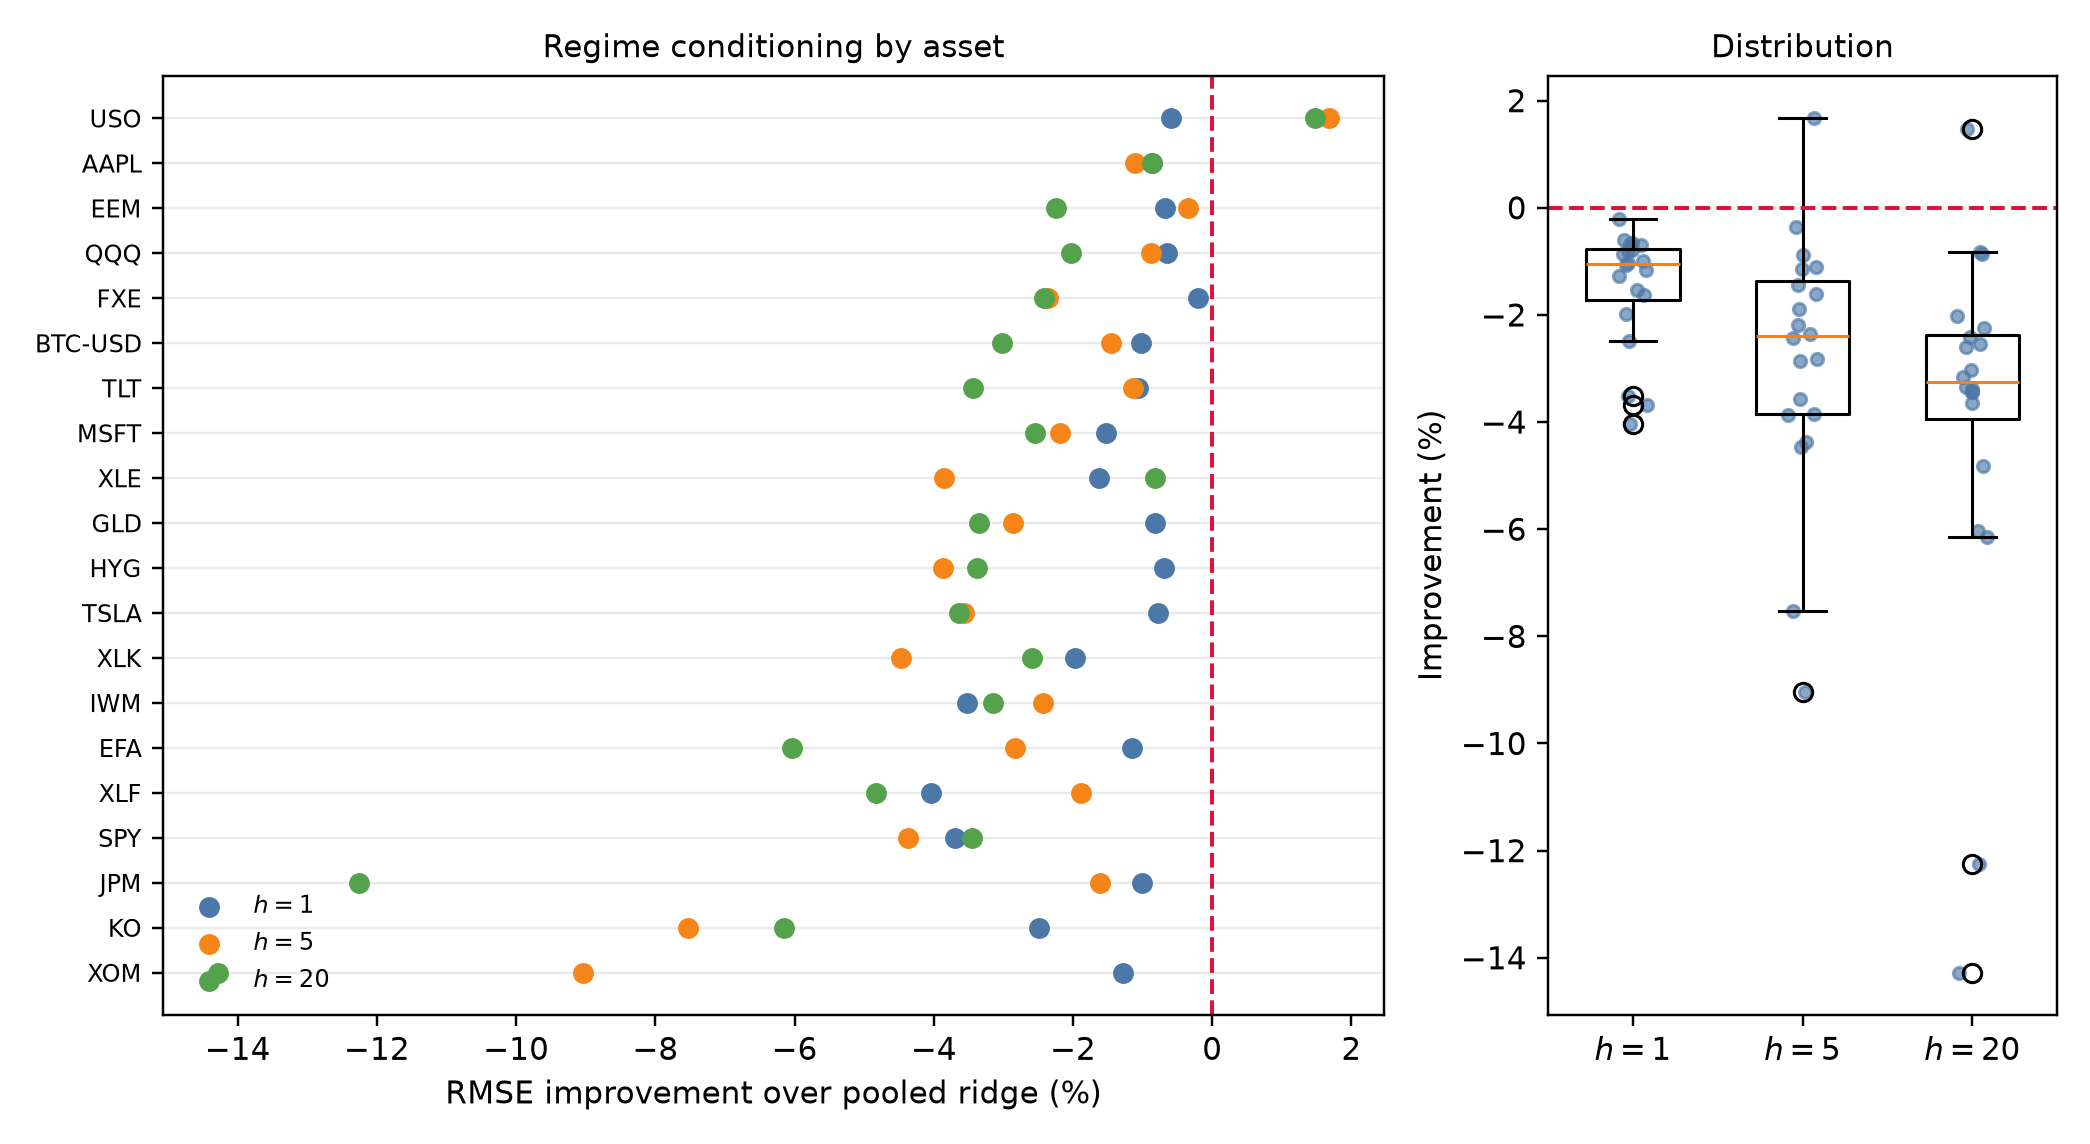
\includegraphics[width=\columnwidth]{figures/multi_asset.png}
  \caption{Cross-asset replication. Each point is one asset at one horizon;
  positive would favour regime conditioning. 58 of 60 cells are negative.}
  \label{fig:multiasset}
  \Description{Left, a dot plot of RMSE improvement for twenty assets at three horizons, with almost all points left of the zero line. Right, box plots of the same distributions by horizon, all centred below zero.}
\end{figure}

A single-asset null carries weak evidence, and SPY is the least favourable series
we could have picked. It is the most liquid and most-studied series available,
and the one where trailing realized volatility tells you most, leaving regime
labels the least room to add anything. We therefore repeat the corrected protocol
on 20 assets spanning broad equity indices, sectors, single names, long-duration
rates, high-yield credit, commodities, FX and crypto, with sample histories of 12
to 21 years.

The null holds across the cross-section. Table~\ref{tab:multiasset} and
Figure~\ref{fig:multiasset} report the regime model's improvement over its
matched pooled ridge: 58 of 60 asset-horizon cells come out negative, with
medians of $-1.05\%$, $-2.39\%$ and $-3.25\%$ at $h = 1, 5, 20$. Of the 60 cells,
37 are significant deteriorations under a Diebold--Mariano test and \emph{none} is
a significant improvement. Both positive cells belong to crude oil (USO), and
neither reaches significance. Correlations between an asset's mean volatility and
the size of the effect stay small and flip sign across horizons ($+0.14$, $+0.20$,
$+0.05$), so we find no sign that regime conditioning pays for more volatile or
less well-behaved assets.

\subsection{The value of regime timing}

\begin{figure}[t]
  \centering
  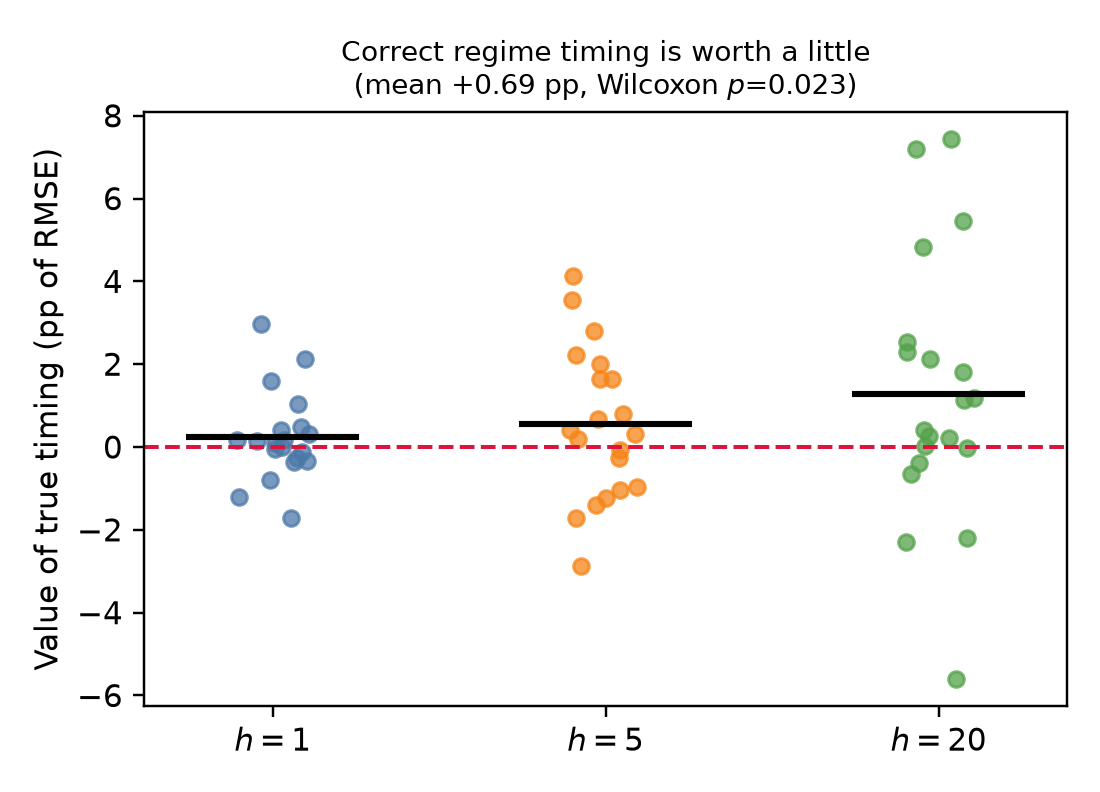
\includegraphics[width=\columnwidth]{figures/multi_asset_gate_shuffle.png}
  \caption{The paired benefit of correct regime timing over a time-shuffled
  gate, in percentage points of RMSE, one point per asset-horizon pair; bars are
  means. The benefit is small, positive on average, and grows with horizon.}
  \label{fig:gateshuffle}
  \Description{Strip plot of the paired benefit of correct regime timing over a time-shuffled gate, by horizon, with means marked. The means are small and positive and grow with horizon.}
\end{figure}

The cross-section measures what the single-asset ablation could only bound
(Figure~\ref{fig:gateshuffle}). Pooling all 60 pairs, correct regime timing beats
shuffled timing in 37 of them. A sign test misses significance at $p = 0.09$,
while the paired magnitudes reach it: the mean benefit is $+0.69$ percentage
points of RMSE, and a Wilcoxon signed-rank test on the paired differences gives
$p = 0.023$. The benefit grows with horizon, from $+0.23$ points at $h{=}1$ to
$+0.54$ at $h{=}5$ and $+1.29$ at $h{=}20$, the pattern we would expect if the
regime state carries information about persistent volatility levels rather than
about tomorrow.

Regime timing therefore carries some value. Two questions remain: whether it
carries enough, and whether the gating mechanism blocks it.

\subsection{Using the regime signal without gating}
\label{sec:variants}

\begin{table}[t]
\caption{Every way of using the regime signal, against the pooled ridge, over 60 asset-horizon pairs. ``Median'' is the median improvement in percent (positive favours the row). ``Wins'' counts pairs where the row beats the pooled ridge; ``sig.\ better'' and ``sig.\ worse'' count Diebold--Mariano rejections at 5\%. No regime variant achieves a single significant improvement in 240 tests, whereas GARCH and EWMA---which ignore regimes entirely---beat the pooled ridge more often than not.}
\label{tab:variants}
\small
\setlength{\tabcolsep}{4pt}
\begin{tabular}{lrrrr}
\toprule
Model & Median & Wins & sig.\ better & sig.\ worse \\
\midrule
Regime gating (full mixture) & -2.30\% & 2/60 & 0 & 37 \\
\quad with time-shuffled gate & -3.14\% & 3/60 & 0 & 40 \\
Regime gating, shrunk to pooled & -0.72\% & 11/60 & 0 & 18 \\
\midrule
Regime posteriors as features & -0.63\% & 4/60 & 0 & 31 \\
HAR & -0.13\% & 26/60 & 7 & 8 \\
GARCH(1,1) & +0.59\% & 39/60 & 4 & 3 \\
EWMA & +0.42\% & 33/60 & 14 & 9 \\
\bottomrule
\end{tabular}
\end{table}


\begin{figure}[t]
  \centering
  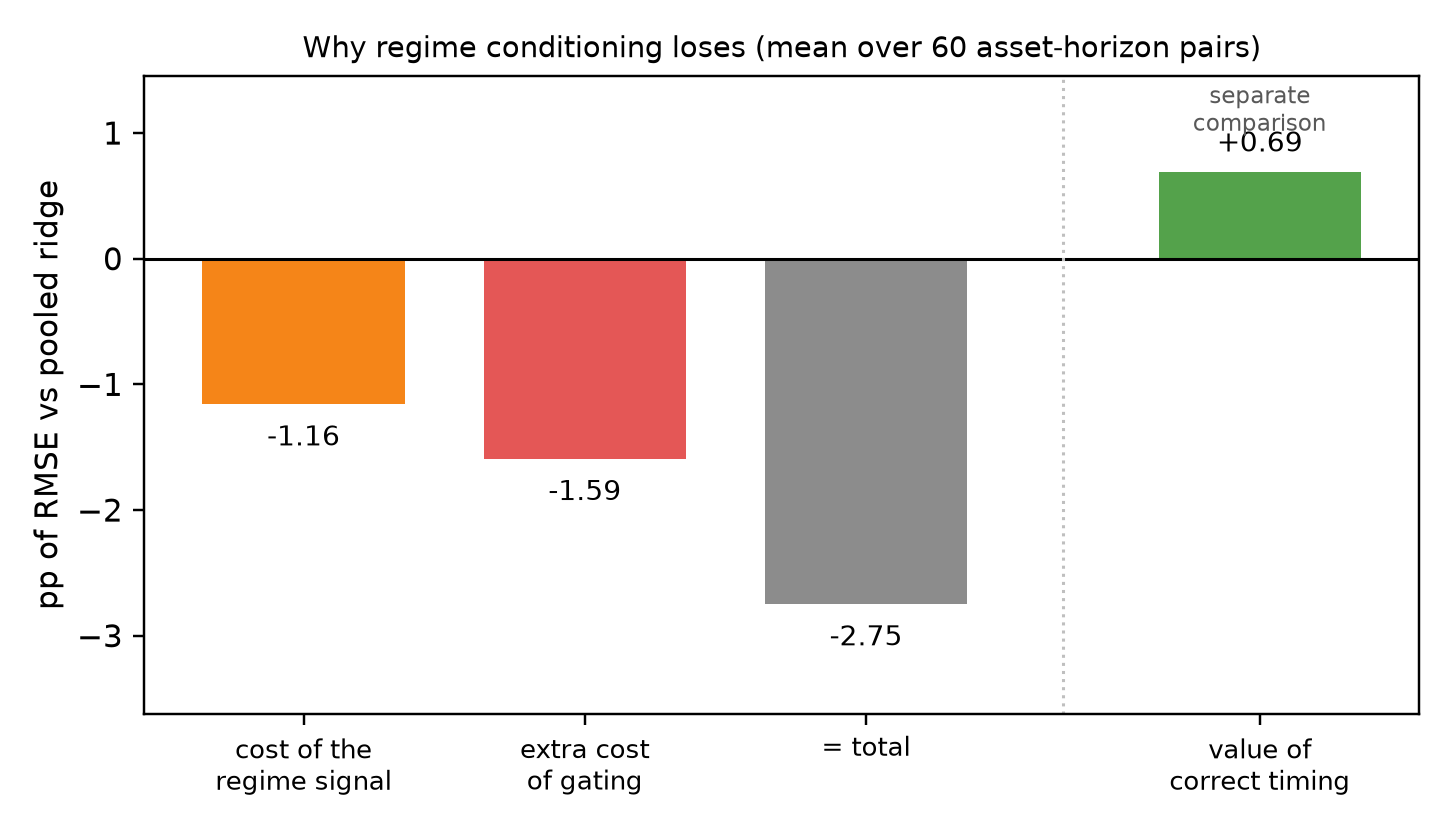
\includegraphics[width=\columnwidth]{figures/cost_decomposition.png}
  \caption{Decomposition of the regime model's loss against the pooled ridge.
  The first two bars are additive by construction. The timing term measures a
  different comparison, gated versus gated-with-shuffled-gate, and forms no part
  of the total.}
  \label{fig:decomposition}
  \Description{Bar chart decomposing the regime model's loss into the cost of the regime signal and the additional cost of gating, which sum to the total, with the value of correct timing drawn separately to its right.}
\end{figure}

If the partition binds, then using the regime posteriors \emph{without}
partitioning should recover the loss. We test the two obvious ways to do that,
both under the same protocol. The first appends the filtered posteriors
$\gamma_t(1),\dots,\gamma_t(K)$ to the feature matrix of a single pooled ridge,
handing the model the regime signal at zero partitioning cost. The second shrinks
the gated mixture toward the pooled fit by a factor selected on the inner
validation block, over a grid containing both endpoints, so it can land on either
extreme.

Neither route rescues the method. Table~\ref{tab:variants} reports all four.
Feature augmentation loses by $0.63\%$ at the median and shrinkage by $0.72\%$,
against $2.30\%$ for full gating. Across the four variants and 240
Diebold--Mariano tests, \emph{none} improves on the pooled ridge at any
conventional level.

Figure~\ref{fig:decomposition} splits the two costs. Injecting the regime signal
at all costs $1.16$ points of RMSE on average (Wilcoxon $p = 2.4\times10^{-9}$);
gating on it rather than conditioning on it costs a further $1.59$ (paired
Wilcoxon $p = 8.7\times10^{-8}$). Both costs are real, and the partition is the
larger, so the mechanism does matter. Remove it and the regime model still trails
a plain ridge.

Two details deserve recording. The shrinkage grid includes $\lambda = 1$, the
pooled ridge itself, and the inner validation block picks it in $15\%$ of folds,
settling on a mean shrinkage of $0.45$ instead. In sample the regime signal looks
useful often enough to get selected; out of sample it does not deliver. Second,
the benchmarks that ignore regimes outperform the ridge we use as the reference:
GARCH(1,1) beats it in 39 of 60 pairs and EWMA in 33. The regime model loses to a
control that is not even the strongest baseline available.

\subsection{What the HMM learns from returns}
\label{sec:simulation}

\begin{table*}[t]
\caption{What the HMM learns from each world. All rows use the identical pipeline. ``Separation'' is the ratio of the highest to the lowest state's mean realized volatility; ``excess persistence'' is the average self-transition probability minus the stationary probability, so zero means states are temporally independent. Persistence is reported with the standard emission vector and again with the 20-day rolling volatility removed; on data with no dynamics at all the first is large and the second is zero, so most of what the usual diagnostic reports is autocorrelation contributed by an overlapping-window feature. ``State recovery'' is the adjusted Rand index against the true latent path where one exists. The final columns are the out-of-sample RMSE improvement from conditioning on the inferred state. Separation and persistence do not distinguish the worlds containing regimes from those that do not; forecasting does.}
\label{tab:simulation}
\small
\begin{tabular}{lccccrrrr}
\toprule
& True & & \multicolumn{2}{c}{Excess persistence} & State & \multicolumn{3}{c}{Forecast improvement} \\
\cmidrule(lr){4-5}\cmidrule(lr){7-9}
Data-generating process & regimes? & Separation & std.\ & no RV$_{20}$ & recovery & $h{=}1$ & $h{=}5$ & $h{=}20$ \\
\midrule
Markov switching (differing dynamics) & \checkmark & 2.80 & +0.406 & +0.139 & 0.13 & -0.07\% & -0.44\% & -1.10\% \\
Markov switching (differing level) & \checkmark & 3.15 & +0.378 & +0.209 & 0.33 & +0.31\% & +0.59\% & +0.09\% \\
GARCH(1,1)-$t$ & $\times$ & 3.00 & +0.392 & +0.105 & -- & -0.75\% & -1.79\% & -2.29\% \\
i.i.d.\ Student-$t$ & $\times$ & 1.60 & +0.261 & +0.002 & -- & -0.09\% & -0.22\% & -0.42\% \\
i.i.d.\ Gaussian & $\times$ & 1.28 & +0.253 & -0.003 & -- & -0.09\% & -0.17\% & -0.59\% \\
\midrule
\textbf{SPY (real data)} & -- & 2.51 & +0.339 & +0.118 & -- & -3.69\% & -4.37\% & -3.45\% \\
\bottomrule
\end{tabular}
\end{table*}


\begin{figure}[t]
  \centering
  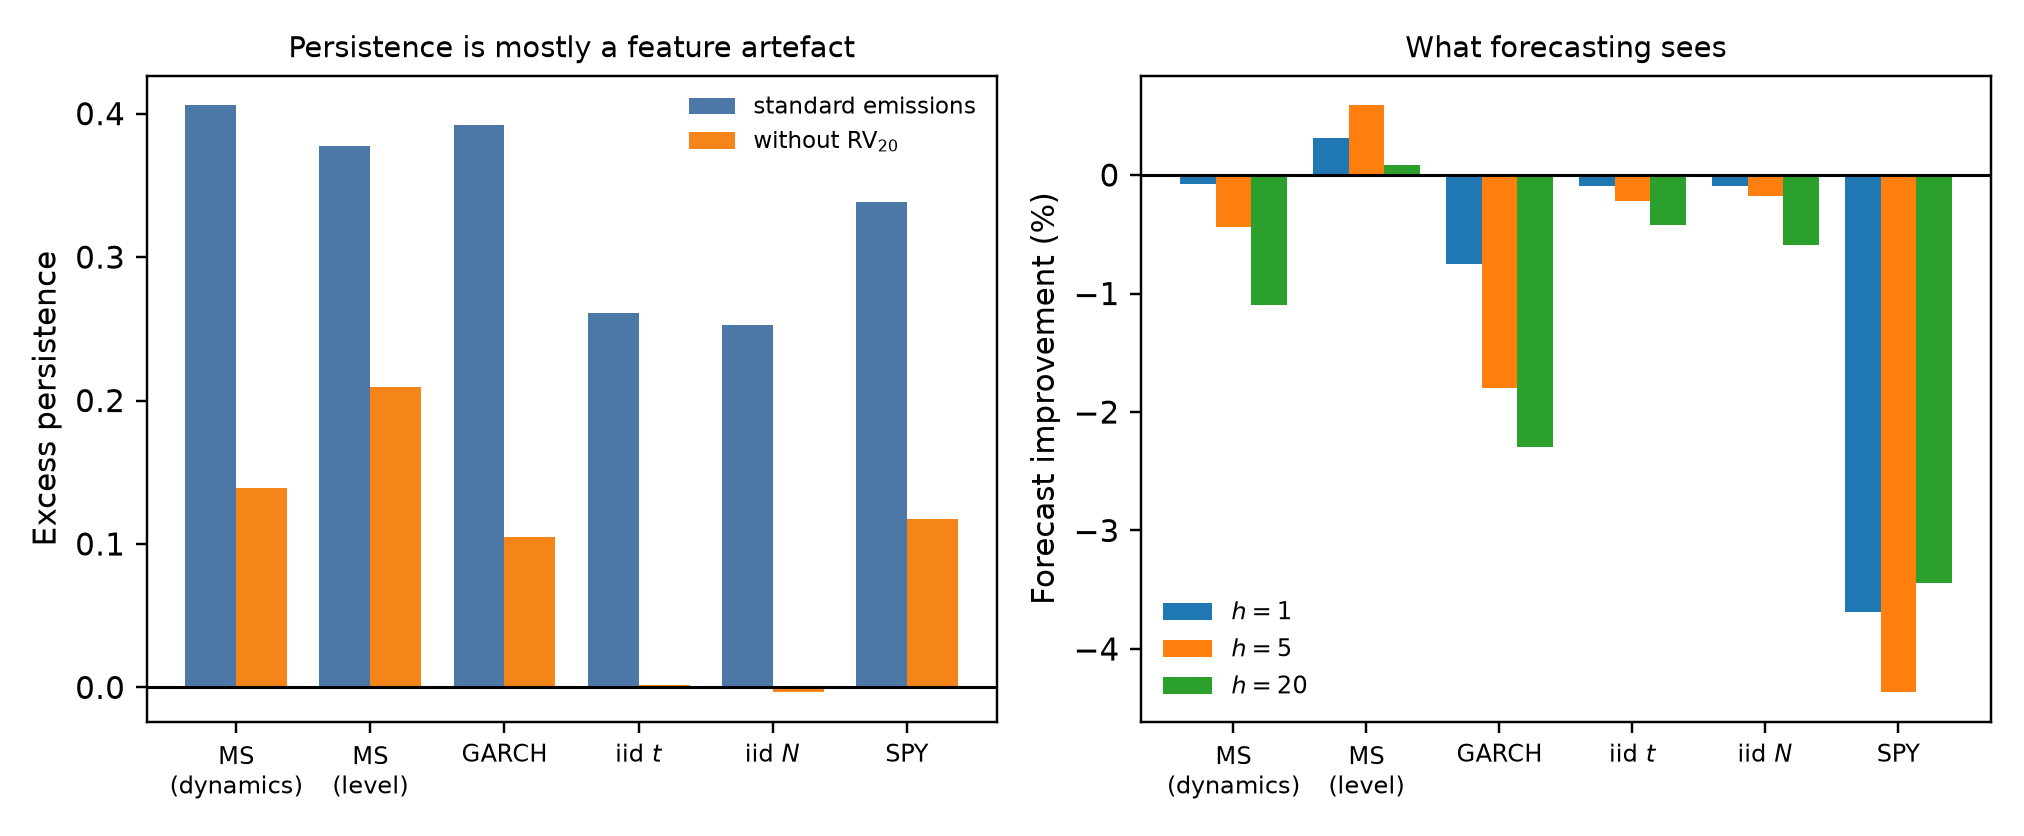
\includegraphics[width=\columnwidth]{figures/simulation.png}
  \caption{Left: apparent regime persistence, with the standard emission vector
  and with the 20-day rolling volatility removed. On i.i.d.\ data the first is
  large and the second is zero. Right: forecast improvement from conditioning on
  the inferred state. Only the right panel separates the worlds that contain
  regimes from those that do not.}
  \label{fig:simulation}
  \Description{Left, paired bars of excess persistence with standard and de-overlapped emissions across five simulated worlds and real data; the second bar is near zero for the worlds without dynamics. Right, forecast improvement by world, positive only where regimes exist.}
\end{figure}

A null result on real data admits two readings on its own: markets may have no
regimes, or our pipeline may fail to find regimes that are there. We settle it by
running the identical pipeline on synthetic data from worlds whose answer we
know. Two have genuine Markov switching, one has persistent continuous volatility
and no discrete states, and two have no dynamics at all. We calibrate the
processes to SPY's unconditional volatility, excess kurtosis and absolute-return
autocorrelation, and we give the GARCH world Student-$t$ innovations so that it
stands in for real returns rather than separating on tail thickness alone.

Table~\ref{tab:simulation} carries four findings.

\paragraph{The usual descriptive diagnostics do not identify regimes.}
State separation reaches $3.00$ in the GARCH world, which contains no discrete
states, against $3.15$ for genuine two-state switching. Show a reader the fitted
means, the transition matrix and a shading plot, and they cannot tell the two
apart. Both resemble the real data.

\paragraph{The emission vector manufactures most of the reported persistence.}
Fit the HMM to i.i.d.\ Gaussian returns, with no
volatility clustering and no regimes, and it reports excess persistence of
$+0.25$, a self-transition probability double the stationary probability. Remove
the 20-day rolling volatility from the emission vector and the figure falls to
$-0.003$, the zero it should have shown all along. Consecutive values of
$\mathrm{RV}^{(20)}$ share 19 of their 20 observations, so the filter reads back
autocorrelation that our own feature construction supplied. The size of the
artefact matches the size of the real signal: of SPY's apparent $+0.339$, only
$+0.118$ survives the removal, and of the GARCH world's $+0.392$, only $+0.105$.
Since ``the inferred regimes are highly persistent'' ranks among the most
reported diagnostics in this literature, we encourage reporting it in the ablated
form.

\paragraph{Only forecasting discriminates, and it places real data with GARCH.}
Regime conditioning helps in the world where regimes exist and differ in level
($+0.31\%$ and $+0.59\%$ at $h=1,5$, both significant across 12 replications),
and hurts in the three worlds where they do not. Real SPY sits with GARCH rather
than with Markov switching. Our pipeline detects regimes when they are present,
so the positive control works, which licenses reading the empirical null as a
statement about markets and not about our implementation.

\paragraph{An unexpected asymmetry.} We built the ``differing dynamics'' world as
the \emph{strongest} case for a regime-conditioned mixture. Its two states share a
volatility level and differ in how fast volatility mean-reverts, so per-regime
experts have different coefficients to learn. Regime conditioning fails there
($-0.44\%$ at $h=5$), and the state-recovery column explains it: the adjusted Rand
index against the true path is $0.13$, against $0.33$ in the world where states
differ in level.

The estimator causes this, not our setup. Baum--Welch maximises the likelihood of
the \emph{emissions}, so it identifies states that differ in their emission
distribution and stays close to blind to states that differ in how the process
evolves. A state that differs in level is one that trailing realized volatility
already reveals, while a state that differs in dynamics is the one that would
carry new information. The estimator excels at finding the regimes least worth
conditioning on and struggles with the ones that would help. Its objective and
the forecasting objective are different, and a correct implementation cannot
close that gap.

\subsection{Two fixes the diagnosis implies}
\label{sec:fixes}

The two failures above, an emission vector that manufactures persistence and an
objective that finds the wrong states, each suggest a remedy. We test both.

\paragraph{Emissions without overlapping windows.}
Replacing the emission vector with volatility-standardised returns
$z_t = r_t / \hat\sigma_{t-1}$, where $\hat\sigma$ is a causal EWMA of past
squared returns, removes the manufactured persistence. Excess persistence on
i.i.d.\ Gaussian returns falls from $+0.301$ to $-0.005$, and on i.i.d.\
Student-$t$ from $+0.297$ to $+0.002$. The diagnostic then starts to
\emph{discriminate}: the GARCH world, holding no discrete states, falls to
$+0.013$, while the two genuine regime worlds hold $+0.065$ and $+0.048$. Under
any process whose only structure is time-varying scale, the standardised series
approaches i.i.d., so persistence that survives points to structure the
volatility level leaves unexplained.

Applied to SPY, the diagnostic returns $-0.001$. Divide out their own volatility
level and real equity returns show \emph{less} regime persistence than a GARCH
process containing no regimes. The apparent regime structure in
Figure~\ref{fig:regimes} is the volatility level and nothing besides. This is the
cleanest statement the paper can make, and we measured it rather than inferring
it.

\paragraph{Estimating the states jointly with the forecast.}

\begin{table}[t]
\caption{Two-stage versus jointly-estimated regimes. Both are RMSE improvement over the same pooled ridge, in percent, averaged over four replications for the synthetic worlds. Both arms use the identical protocol: embargoed walk-forward splits, $K$ and the ridge penalty selected on the inner validation block, and causal prediction. Joint estimation is much better where regimes exist and differ in level, no better where they differ only in dynamics, and markedly worse where there are no regimes to find.}
\label{tab:joint}
\small
\setlength{\tabcolsep}{4pt}
\fitwidth{%
\begin{tabular}{lrrrrrr}
\toprule
& \multicolumn{3}{c}{Two-stage} & \multicolumn{3}{c}{Joint} \\
\cmidrule(lr){2-4}\cmidrule(lr){5-7}
Data-generating process & $h{=}1$ & $h{=}5$ & $h{=}20$ & $h{=}1$ & $h{=}5$ & $h{=}20$ \\
\midrule
Markov switching (level) & +0.37 & +0.72 & -0.66 & +2.62 & +3.91 & -6.97 \\
Markov switching (dynamics) & +0.13 & +0.14 & -0.70 & -1.66 & -0.98 & -4.54 \\
GARCH(1,1)-$t$ \quad(no regimes) & -0.98 & -3.52 & -6.44 & -4.80 & -7.38 & -11.84 \\
\midrule
\textbf{SPY (real data)} & -1.13 & -4.58 & -3.56 & -8.10 & -11.41 & -2.72 \\
\bottomrule
\end{tabular}%
}
\end{table}


If Baum--Welch optimises the wrong objective, the fix is to make the emission the
predictive density itself,
$p(y_t \mid x_t, z_t{=}k) = \mathcal{N}(\beta_k' x_t, \sigma_k^2)$, and estimate
$\beta$, $\sigma$ and the transition matrix jointly by EM. Hamilton
\cite{hamilton1989} introduced this Markov-switching regression, so the estimator
is not new. We contribute the controlled comparison against the two-stage
pipeline, on data whose regimes we control, giving both arms the same protocol:
embargoed splits, $K$ and the ridge penalty selected on the same inner validation
block, and a horizon-aware causal filter for out-of-sample prediction.

The results split three ways.

Joint estimation gains a great deal where regimes exist and the estimator can
identify them. On the level-switching world it returns $+2.62\%$ and $+3.91\%$ at
$h=1,5$ against the two-stage pipeline's $+0.37\%$ and $+0.72\%$, a sevenfold
difference. Our diagnosis holds up that far: the objective mismatch is real, and
removing it recovers much more of the available signal.

Joint estimation fails to rescue the dynamics-switching world, the case we
expected it to fix. It loses there at every horizon and beats the two-stage
pipeline in 1 of 12 replications. We predicted the opposite. The implication runs
further than what we set out to demonstrate: states that share a volatility level
and differ in how volatility evolves appear unrecoverable from a return series by
\emph{either} estimator. That bounds what any regime detector reading returns
alone can deliver, and it constrains the data rather than the choice of
objective.

In the GARCH world and in real data, holding no regimes, joint estimation trails
the two-stage pipeline by a wide margin ($-4.80\%$ and $-8.10\%$ at
$h=1$). Give a model $K$ times the parameters and nothing to find, and the extra
flexibility overfits. This matches the emission diagnostic above: SPY holds no
residual regime structure for a better estimator to exploit, so the more powerful
estimator does more damage.

One practical recommendation follows. Run the standardised-emission diagnostic
first. If it returns near zero, as it does for SPY, no regime machinery of any
sophistication will help; condition on volatility continuously and stop. If it
returns something well above zero, prefer joint estimation to the two-stage
pipeline, and expect it to find only regimes that differ in level.

\subsection{Model confidence sets}
\label{sec:mcs}

\begin{table}[t]
\caption{Model Confidence Set \cite{hansen2011mcs} at the 90\% level, computed separately for each of the 60 asset-horizon pairs with a stationary block bootstrap at block length $h$. Entries are the percentage of pairs in which the model survives into the set of models that cannot be distinguished from the best. Regime-conditioned models are in bold. Unlike the pairwise tests, this accounts for the full set of competitors simultaneously.}
\label{tab:mcs}
\small
\begin{tabular}{lrr}
\toprule
Model & MSE & QLIKE \\
\midrule
Ridge (pooled) & 75\% & 67\% \\
HAR & 52\% & 65\% \\
GARCH(1,1) & 78\% & 88\% \\
EWMA & 77\% & 85\% \\
Gradient boosting (pooled) & 18\% & 43\% \\
\midrule
\textbf{Regime gating} & 28\% & 42\% \\
\textbf{Regime as features} & 40\% & 55\% \\
\textbf{Regime gating, shrunk} & 60\% & 72\% \\
\textbf{Regime gating, GBM experts} & 15\% & 35\% \\
\bottomrule
\end{tabular}
\end{table}


Our tests so far run pairwise. Against a dozen competitors that asks too little:
a model can avoid losing to any single rival and still drop out once all of them
compete at once. The Model Confidence Set \cite{hansen2011mcs} returns the set of
models that cannot be distinguished from the best, the object our claim concerns.
We compute it separately for each of the 60 asset-horizon pairs at the 90\%
level, using a stationary block bootstrap \cite{politis1994} with block length
$h$ to preserve the dependence that overlapping targets induce.

Table~\ref{tab:mcs} reports how often each model survives, and the ordering
leaves no ambiguity. GARCH(1,1) and EWMA, neither of which knows anything about
regimes, survive in $78\%$ and $77\%$ of pairs under MSE and in $88\%$ and $85\%$
under QLIKE. The full regime mixture survives in $28\%$ and $42\%$. Boosted regime
experts, the most elaborate model we fit, survive least often of all, at $15\%$
and $35\%$.

The shrunk mixture holds up better than the other regime variants, at $60\%$ and
$72\%$, and the reason deflates the result: shrinkage selected on the inner split
pulls it most of the way back toward the pooled ridge, so the ridge is what
survives. Across all four regime variants and both losses, no variant survives as
often as the simplest volatility model in the comparison.

\subsection{Equivalence bounds}
\label{sec:equivalence}

\begin{table}[t]
\caption{Equivalence bounds. For each asset-horizon pair we form a 95\% confidence interval on the regime model's RMSE improvement over the pooled ridge and report the upper limit, i.e.\ the largest improvement the data cannot exclude. A negative bound means \emph{no} improvement of any size is consistent with the data at 95\%. This is the statement a null result requires: failing to reject equal accuracy is also what an underpowered test produces.}
\label{tab:equivalence}
\small
\begin{tabular}{llrrr}
\toprule
Variant & Horizon & Median bound & Worst case & Bound $<0$ \\
\midrule
Regime gating (full mixture) & $h=1$ & -0.12\% & +0.80\% & 13/20 \\
 & $h=5$ & -0.47\% & +6.14\% & 13/20 \\
 & $h=20$ & -0.11\% & +10.34\% & 11/20 \\
\midrule
Regime posteriors as features & $h=1$ & -0.02\% & +0.64\% & 11/20 \\
 & $h=5$ & -0.15\% & +4.39\% & 11/20 \\
 & $h=20$ & +0.22\% & +3.89\% & 9/20 \\
\midrule
Regime gating, shrunk to pooled & $h=1$ & +0.13\% & +0.94\% & 6/20 \\
 & $h=5$ & +0.46\% & +6.52\% & 7/20 \\
 & $h=20$ & +0.50\% & +6.94\% & 5/20 \\
\bottomrule
\end{tabular}
\end{table}


An underpowered test also fails to reject equal accuracy, so that failure on its
own establishes nothing. Since our central claim is a null, we carry the burden of
showing the study could have detected an effect had one existed.

Table~\ref{tab:equivalence} reports, for each asset-horizon pair, the upper limit
of a 95\% confidence interval on the regime model's RMSE improvement over the
pooled ridge: the largest improvement the data leave open. We build the interval
on the same HAC-corrected loss differential as the Diebold--Mariano tests and map
it monotonically onto the RMSE percentage scale.

In the median pair that upper limit comes out negative at every horizon, so no
improvement of any size survives at 95\%. The bounds tighten at $h{=}1$, where
even the least informative asset rules out improvements above $0.80\%$. They
loosen at longer horizons, and the weakest single case at $h{=}20$ rules out only
improvements above $10.3\%$, because overlapping 20-day targets leave far fewer
effective observations and the HAC correction reflects that. We claim no tight
bound at $h{=}20$ for every asset. We claim that at $h{=}1$, and in the median
case at all horizons, we measured the null instead of failing to find one.

\subsection{Seed sensitivity}
\label{sec:seeds}

\begin{table}[t]
\caption{Sensitivity to the HMM's random initialization. Ten seeds, everything else fixed. $\Delta$\% is improvement over the (deterministic) pooled ridge. The spread across seeds is comparable to the effect size the comparison is trying to resolve.}
\label{tab:seed}
\small
\fitwidth{%
\begin{tabular}{lrrrrr}
\toprule
Horizon & Pooled ridge & RMSE mean & RMSE s.d. & $\Delta$\% min & $\Delta$\% max \\
\midrule
$h=1$ & 0.006968 & 0.007114 & 0.000081 & -3.69 & -0.18 \\
$h=5$ & 0.004719 & 0.004948 & 0.000059 & -6.71 & -1.94 \\
$h=20$ & 0.004867 & 0.005043 & 0.000046 & -5.19 & -2.36 \\
\bottomrule
\end{tabular}%
}
\end{table}


\begin{figure}[t]
  \centering
  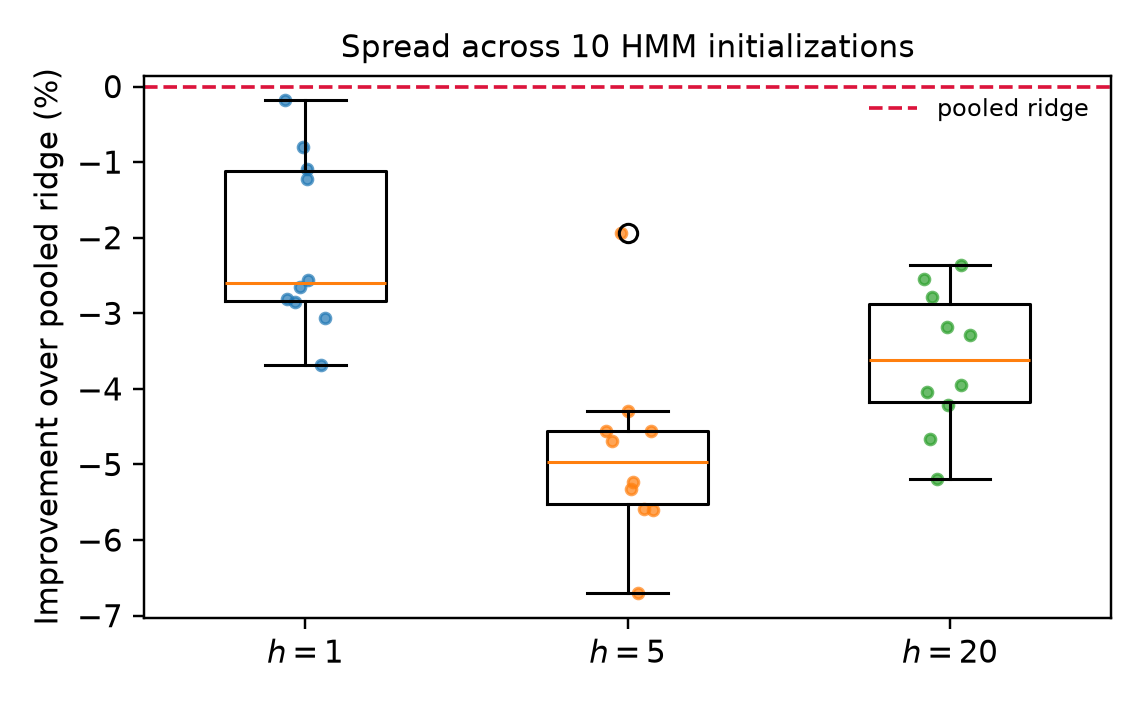
\includegraphics[width=0.85\columnwidth]{figures/seed_robustness.png}
  \caption{Improvement over the pooled ridge across ten HMM initializations.
  Every seed is negative, but the spread is wide enough that a single run could
  report anything within it.}
  \label{fig:seeds}
  \Description{Box plot with overlaid points of the improvement over pooled ridge across ten HMM initialisations at three horizons. Every point lies below the zero line.}
\end{figure}

Baum--Welch maximizes a non-convex likelihood. Table~\ref{tab:seed} and
Figure~\ref{fig:seeds} report the spread of out-of-sample RMSE across ten random
initializations, holding everything else fixed. That range matches the differences
the model comparison sets out to resolve, and the seed also shifts the number of
regimes that nested selection picks. A single-seed comparison between a regime
model and a baseline therefore tells you little, and single-seed results remain
the norm in this literature.

Every seed leaves the regime model behind the pooled ridge, so our conclusion
survives the draw. The spread shows that the \emph{magnitude} any one run reports
belongs to that run and not to the method, and that a study reporting a small
positive effect from a single seed has measured nothing. Report the seed
distribution as a matter of course.

\subsection{The regimes are real}

\begin{figure}[t]
  \centering
  
\includegraphics[width=\columnwidth]{figures/regime_shading.png}
  \caption{Out-of-sample filtered regimes for the $K{=}3$ model at $h{=}5$.
  Shading marks contiguous hard-state segments with opacity proportional to
  posterior confidence. Top: cumulative log return. Bottom: trailing realized
  volatility. The high-volatility state aligns with 2011, 2015--16, 2018, 2020
  and 2022.}
  \label{fig:regimes}
  \Description{Two stacked time-series panels for SPY from 2011 to 2026, cumulative log return above and trailing realized volatility below, shaded by inferred regime. The high-volatility shading coincides with the 2011, 2018, 2020 and 2022 volatility spikes.}
\end{figure}

\begin{table}[t]
\caption{What the inferred regimes do capture ($K{=}3$, $h{=}5$, out-of-sample). ``Stress'' is the top decile of realized volatility over the forecast window, so the unconditional rate is 10\%. Lift is the ratio of the within-regime rate to that base rate. The high-volatility state occupies a sixth of the sample and contains nearly three-fifths of all stress events---the regimes are genuinely informative, just not incrementally so for the conditional mean.}
\label{tab:regimes}
\small
\fitwidth{%
\begin{tabular}{lrrrrr}
\toprule
Regime & \% of time & Mean RV$^{(20)}$ & P(stress) & Lift & \% of all stress \\
\midrule
Low vol & 47.3 & 0.00623 & 0.021 & 0.21 & 9.8 \\
Mid vol & 36.4 & 0.00884 & 0.087 & 0.87 & 31.5 \\
High vol & 16.3 & 0.01707 & 0.360 & 3.60 & 58.7 \\
\bottomrule
\end{tabular}%
}
\end{table}


The HMM does find structure. Figure~\ref{fig:regimes} shows the filtered
high-volatility state tracking recognized stress episodes, and doing so causally,
without lookahead. The fits behave well: across all 15 folds no state collapses,
the canonical volatility ordering stays monotone in every fold for
$K \in \{2,3\}$, and mean self-transition probabilities reach $0.93$, $0.81$ and
$0.68$ for $K = 2, 3, 4$, so the inferred states persist instead of flickering.

Table~\ref{tab:regimes} quantifies it, and the numbers are large. The
high-volatility state occupies $16\%$ of the out-of-sample period and contains
$59\%$ of all volatility spikes. Conditional on sitting in it, the probability of
a top-decile spike over the next week is $36\%$ against an unconditional $10\%$, a
lift of $3.6\times$. The causal HMM works as a stress \emph{classifier}.

This finding takes the paper's result to its sharpest form, and it admits a
direct test. If the regime label re-encodes trailing volatility, then trailing
volatility should recover it. Regressing the filtered hard state on the three HAR
components alone, with no other features and no HMM, recovers it with $95.7\%$
accuracy against a $46.2\%$ base rate. (We fit this in sample as a description,
not a forecast. The question is whether the regime variable is a function of
information already present, not whether anyone can predict it.)

That mechanism drives Section~\ref{sec:variants}. The HMM state encodes, at three
noisy levels refitted once a year, a quantity every model in the comparison
already reads continuously and without estimation error. It cannot supply
information the model lacks, and it does supply estimation noise, which is why
feature augmentation loses even with no partition to pay for. Gating then adds a
second and larger cost.

This distinction matters in practice. Regime labels may still earn their place in
communication, risk limits or position sizing, and a $3.6\times$ lift on stress
is a usable signal for those purposes. Our result covers one thing: they do not
improve the conditional mean of realized volatility.

%======================================================================
\section{A Checklist}
%======================================================================

The audit that produced this paper reduces to a small number of checks that we
would encourage as standard for regime-switching forecasting work:

\begin{enumerate}
  \item \textbf{Verify the target varies with the horizon.} Compare the marginal
    distributions of $y^{(h)}$ across $h$. If they are identical, the target is
    a single-period quantity at longer lead, not a multi-horizon forecast.
  \item \textbf{Use filtered, not smoothed, state probabilities}, and verify it
    by checking that $\gamma_t$ holds unchanged when you delete data after $t$
    deleted.
  \item \textbf{Purge the training window by the horizon.}
  \item \textbf{Select hyperparameters inside the training window.} If the
    number of regimes is chosen on the test score, the test score is no longer
    an estimate of out-of-sample performance.
  \item \textbf{Give the baseline the same care as the model:} standardization,
    tuned regularization, and access to the same features. Include HAR and
    GARCH for volatility targets.
  \item \textbf{Run a gate-shuffle ablation}, and compare what correct timing
    buys against what the conditioning mechanism costs. Both quantities are
    measurable on the same scale, and only their difference is the result.
    Interpret the ablation across many series: on a single asset it is too noisy
    to distinguish ``no signal'' from ``signal too small to pay for itself''.
  \item \textbf{Check that an ablation is not a duplicate.} Ours were: two of the
    four arms in our first design returned bitwise-identical numbers.
  \item \textbf{Relabel states canonically before pooling across folds}, or every
    per-regime table mixes different regimes together without warning.
  \item \textbf{Check the regime variable is not redundant} with a feature the
    model already has. Regress the inferred state on your existing volatility
    features: ours was $95.7\%$ recoverable, and nothing downstream could fix
    that.
  \item \textbf{Report persistence with overlapping-window emissions removed.}
    An HMM fitted to i.i.d.\ noise reports substantial regime persistence if its
    emission vector contains a rolling statistic. Refit without it and report
    both numbers.
  \item \textbf{Validate on a simulated world with known regimes.} If
    conditioning does not help where regimes provably exist, the architecture is
    at fault and no amount of real data will reveal it. If it does help there and
    not on real data, that is evidence about markets rather than about code.
  \item \textbf{Test the signal without the mechanism.} Before concluding that
    gating is what fails, feed the posteriors in as plain features. The two
    diagnoses imply different remedies.
  \item \textbf{Report the seed distribution}, not a single run.
  \item \textbf{Test significance} with a HAC-corrected Diebold--Mariano test and
    correct for the number of comparisons.
  \item \textbf{Report what your null excludes,} not just that you failed to
    reject. An equivalence bound distinguishes a measured null from an
    underpowered one.
\end{enumerate}

%======================================================================
\section{Limitations}
%======================================================================

Our result holds along specific dimensions, and we would rather not
overgeneralize from them.

\emph{Asset universe.} We cover 20 liquid, exchange-traded instruments. They span
asset classes, but all of them trade liquidly and carry long histories. Illiquid
or short-history assets, and instruments whose volatility follows scheduled
events instead of persistence, fall outside our sample.

\emph{Expert families.} We test ridge and gradient-boosted experts. The gating
cost depends on the family: large and significant for ridge, indistinguishable
from zero for boosting (Section~\ref{sec:nonlinear}). The decomposition in
Section~\ref{sec:variants} therefore describes linear experts, and we would not
assume it generalises. Across both families the regime-conditioned model loses to
a plain pooled ridge.

\emph{One family of regime detector.} We use a Gaussian HMM on a
three-dimensional emission vector, every component of which is a function of past
returns. A detector reading information outside the trailing-volatility span,
such as order flow, options-implied measures or macroeconomic releases, would
escape the redundancy that Section~\ref{sec:variants} documents in ours. We
regard that as the most promising direction the paper points at, and the
redundancy diagnostic of Section~\ref{sec:variants} as the first check such work
should report.

\emph{Economic evaluation is narrow.} We test volatility targeting and VaR one
asset at a time. Regime information may matter more for problems our setup cannot
see: cross-asset allocation, where correlations shift with regime
\cite{guidolin2007}, or drawdown control, where the timing of a regime call
outweighs the accuracy of a conditional mean.

\emph{Gaussian HMM with a small emission vector.} Richer emissions, non-Gaussian
observation densities or duration-dependent transitions could recover regimes
less redundant with trailing volatility.

\emph{Conditional mean only.} We evaluate point forecasts. Regime models produce
predictive \emph{distributions}, and their value may sit in tail quantiles or
density forecasts, which our loss functions leave unprobed.

\emph{Fixed evaluation window.} Our results cover 2011--2026 out of sample. That
period contains major stress episodes and remains one realization of history.

\emph{Pairwise testing.} Section~\ref{sec:mcs} reports a Model Confidence Set, but
our headline comparisons use Holm-corrected pairwise Diebold--Mariano tests
against a fixed reference model, since our claims name specific benchmarks. The
two agree here, and readers who prefer the joint object should read
Table~\ref{tab:mcs} as the primary evidence.

%======================================================================
\section{Conclusion}
%======================================================================

We set out to show that causally-inferred market regimes improve volatility
forecasting, and found that they do not. Against well-specified benchmarks,
with an embargoed split and hyperparameters selected inside the training window,
a pooled ridge beats the HMM regime-conditioned version of itself in 58 of 60
asset-horizon pairs, and loses significantly in none.

The reason it fails matters more, and it differs from the one we first reached
for. The regime signal exists: the inferred high-volatility state predicts stress
with a $3.6\times$ lift, and correct timing earns a measurable $0.69$ points of
RMSE. We first read the gating mechanism as too expensive, which predicts that
feeding the posteriors in as plain features should work. That variant loses too,
by $1.16$ points before any gating cost arrives. Features the model already holds
recover the regime state with $95.7\%$ accuracy, so every route of injecting it
supplies estimation noise and no information, and gating adds a further $1.59$
points.

The distinction changes what anyone should do next. ``The mechanism is too
expensive'' invites better mechanisms. ``The variable duplicates what you already
condition on'' invites a different regime detector, one reading information
outside the trailing-volatility span, or none at all. Without testing the
non-gating variants we could not have separated the two, and we would have
published the wrong recommendation.

The conclusion held on every axis we pushed it: nonlinear experts, a Model
Confidence Set weighing all competitors at once, and a decision-relevant loss.
That last case softens the picture, and we report it because it is true and
because it shows that the ranking under squared error need not be the ranking
that matters. Under volatility targeting the regime models become
indistinguishable from the pooled ridge instead of trailing it. The
recommendation stands, since the models ignoring regimes stay significantly ahead
of both.

We also recovered a significant positive result by reintroducing four common
evaluation shortcuts. Negative results in forecasting resist interpretation on
their own, because anyone can attribute a null to insufficient tuning. Tracing
the path from a null to a significant positive and back makes the failure mode
concrete, and we hope harder to reproduce by accident.

\section*{Reproducibility}

Three entry points produce every result from raw data: the study driver, the
protocol ablation and the seed sweep. Every table and figure in this paper comes
from the stored artifacts programmatically, with nothing transcribed by hand.
This buys more than tidiness. The project this paper grew out of carried a
hand-copied results table whose numbers matched no artifact in the repository,
and automating the path from artifact to table is what caught it.

Tests cover the correctness claims that matter, including the lookahead check
described in Section~\ref{sec:protocol-def}: we recompute the filtered
probabilities on truncated inputs and assert equality, so a regression to
smoothed posteriors fails the suite instead of improving the results without
anyone noticing. Code, configuration and artifacts accompany the submission.


%======================================================================
\appendix
\section{Additional robustness checks}
\label{sec:appendix}
%======================================================================

Both checks below confirm the conclusions of Section~\ref{sec:results} without altering them, and are reported here to keep the main text on the argument rather than on its corroboration.

\subsection{Nonlinear experts}
\label{sec:nonlinear}

Our experts are linear, which invites the objection that a regime label earns its
keep only when it gates different functional forms. We therefore repeat the
comparison with gradient-boosted experts, pooled and gated, holding $K$ fixed at
3.

The objection fails, though for a reason we did not expect. Gradient boosting
scores \emph{worse} than ridge at this task, by a median $6.03\%$ in pooled RMSE,
and it wins $0$ of $60$ pairs. That matches the long-standing observation that
realized volatility runs close to linear in its own lagged components, the fact
HAR builds on \cite{corsi2009}. Gating those experts leaves them at $6.29\%$, so
the branch stays uncompetitive whatever we do with the regime signal.

The gating cost carries the interest here. With ridge experts, gating costs
$2.30$ points (Wilcoxon $p = 1.6\times10^{-10}$); with boosted experts it costs
$0.11$ points, indistinguishable from zero ($p = 0.37$). An earlier draft of ours
predicted the reverse, reasoning that more flexible experts would raise the
partition cost since each one fits on a fraction of the window. That prediction
was wrong. A boosted model can represent regime-dependent behaviour internally
through its splits, which makes explicit gating redundant instead of costly, and
its own variance swamps any marginal partition effect. We record the failed
prediction because it bears on the paper's method: the partition cost belongs to
the expert family and does not generalise, so our decomposition in
Section~\ref{sec:variants} describes linear experts.

\subsection{Economic evaluation}
\label{sec:economic}

\begin{table}[t]
\caption{Economic evaluation, median over 20 assets. Volatility targeting sizes a position at $\sigma^{\text{target}}/\hat\sigma_t$ for a 10\% annualised target; the reported error is $|\text{realised}-\text{target}|$ annualised volatility, so lower is better. VaR is at the 5\% level with the forecast-to-quantile scaling calibrated by filtered historical simulation on a trailing window, evaluated at $h{=}1$ where the realised signed return is unambiguous. ``Pass CC'' is the share of assets passing Christoffersen conditional coverage at 5\%.}
\label{tab:economic}
\small
\setlength{\tabcolsep}{4pt}
\begin{tabular}{lrrrrr}
\toprule
& \multicolumn{3}{c}{Vol-target error} & \multicolumn{2}{c}{VaR (5\%, $h{=}1$)} \\
\cmidrule(lr){2-4}\cmidrule(lr){5-6}
Model & $h{=}1$ & $h{=}5$ & $h{=}20$ & Rate & Pass CC \\
\midrule
Ridge (pooled) & 0.0375 & 0.0104 & 0.0049 & 0.052 & 95\% \\
HAR & 0.0347 & 0.0099 & 0.0040 & 0.052 & 95\% \\
GARCH(1,1) & 0.0337 & 0.0093 & 0.0031 & 0.052 & 90\% \\
EWMA & 0.0350 & 0.0109 & 0.0040 & 0.052 & 75\% \\
Gradient boosting (pooled) & 0.0389 & 0.0116 & 0.0074 & 0.053 & 65\% \\
\midrule
\textbf{Regime gating} & 0.0370 & 0.0111 & 0.0056 & 0.053 & 95\% \\
\textbf{Regime as features} & 0.0369 & 0.0119 & 0.0056 & 0.053 & 95\% \\
\textbf{Regime gating, shrunk} & 0.0360 & 0.0099 & 0.0046 & 0.051 & 95\% \\
\textbf{Regime gating, GBM experts} & 0.0392 & 0.0130 & 0.0085 & 0.053 & 65\% \\
\bottomrule
\end{tabular}
\end{table}


Nobody uses a volatility forecast to minimise squared error. A model with worse
RMSE but a $3.6\times$ lift on stress classification could still feed a risk
system better, and that would give this paper its one positive finding. We test
two standard uses.

\emph{Volatility targeting.} We size the position at
$\sigma^{\text{target}}/\hat\sigma_t$ for a $10\%$ annualised target
\cite{moreira2017} and measure how far realized volatility lands from that
target. The exercise assumes no distribution and the loss reads off the result.

\emph{Value-at-Risk.} We convert the forecast to a $5\%$ quantile by filtered
historical simulation on a trailing window, so the scaling uses past information
only, then test coverage with Kupiec \cite{kupiec1995} and Christoffersen
\cite{christoffersen1998}.

The economic evidence in Table~\ref{tab:economic} runs softer than the
statistical evidence, and in one respect kinder to regime conditioning. On
volatility targeting no regime variant differs significantly from the pooled
ridge. The full mixture comes out marginally worse (paired Wilcoxon $p = 0.053$)
and the shrunk mixture marginally better ($p = 0.34$), neither conclusive. Under
a decision-relevant loss the regime models become \emph{indistinguishable} from
the pooled ridge instead of trailing it, as they do under RMSE. That difference
between loss functions deserves recording.

It still builds no case for regime conditioning, because the regime-free
benchmarks beat both. GARCH(1,1) cuts the volatility-targeting error relative to
the pooled ridge at every horizon ($p < 10^{-4}$, better in 43 of 60 pairs), and
HAR does the same ($p = 0.006$). The regime models tie with the pooled ridge, and
the pooled ridge is not the frontier.

The VaR results tell us little about model quality, and we report that rather
than dressing them as support. Filtered historical simulation recalibrates the
forecast-to-quantile scaling on a trailing window, absorbing level errors, so
every non-degenerate model attains near-nominal coverage ($5.1$--$5.3\%$) and
passes conditional coverage in $85$--$95\%$ of assets. Only the random walk in
realized volatility fails, passing in $10\%$ of assets, and it fails because its
forecasts swing rather than because it sits at the wrong level. Models separate
on the average VaR level at matched coverage, meaning how much capital the
forecast ties up, and there the regime mixture ranks least efficient among the
well-calibrated models ($-0.0211$ against $-0.0207$ for GARCH). That margin is
small and we build no argument on it.


\bibliographystyle{ACM-Reference-Format}
\bibliography{references}

\end{document}
